\documentclass[12pt]{amsart}

\addtolength{\hoffset}{-2.25cm}
\addtolength{\textwidth}{4.5cm}
\addtolength{\voffset}{-2.5cm}
\addtolength{\textheight}{5cm}
\setlength{\parskip}{0pt}
\setlength{\parindent}{15pt}
\usepackage{listings}
\usepackage{amsthm}
\usepackage{amsmath}
\usepackage[spanish]{babel}
\usepackage[sort&compress, numbers]{natbib}
\usepackage{amssymb}
\usepackage[utf8]{inputenc}
\usepackage[colorlinks = true, linkcolor = thistle, citecolor = thistle, final]{hyperref}
\usepackage{listings}
\usepackage{ragged2e}
\usepackage{subcaption} 
\usepackage{minted}
\usemintedstyle{borland}
\usepackage{multicol}
\usepackage{listings}
\usepackage{xcolor}
\usepackage{graphicx}
\usepackage[sort&compress, numbers]{natbib}
\usepackage{xcolor}
\usepackage{listings}
\usepackage{ragged2e}
\usepackage{graphicx}
\usepackage[sort&compress, numbers]{natbib}
\usepackage{xcolor}
\usepackage{listings}
\usepackage{ragged2e}
\hypersetup{
    colorlinks=true,
    linkcolor=violet,
    filecolor=violet,     
    urlcolor=violet,
    citecolor=violet,
}
\usepackage{graphicx}
\usepackage[sort&compress, numbers]{natbib}
\usepackage{xcolor}
\usepackage{listings}
\usepackage{ragged2e}

\lstset{style=mystyle}
\usepackage{graphicx}
\usepackage{multicol}
\usepackage{ marvosym }
\newcommand{\ds}{\displaystyle}


\pagestyle{myheadings}

\setlength{\parindent}{0in}
\begin{document}

\pagestyle{empty}



\thispagestyle{empty}

{\scshape Simulación} \hfill {\scshape \Large Tarea 11: Algoritmo genético} \hfill  {\scshape 12/May/2021}
\author{C. María Montemayor Palos}
\maketitle
\hrule
\hrule
\bigskip
\section{Objetivo}
El objetivo es graficar el porcentaje de soluciones de Pareto como función del número de funciones objetivo para $k \in [2, 8]$ en pasos de dos con diagramas de violín combinados con diagramas de caja-bigote, verificando las diferencias observadas sean estadísticamente significativas.

\section{Metodología}
Para efectos de la tarea \cite{dra} se utiliza el programa R versión 4.0.4 \cite{R} para Windows. Esta tarea se basa en el método de análisis de Pareto, el cual permite obtener resultados mediante la optimización multiobjetivo con ayuda de criterios de utilidad en donde permite discernir y proporcionar una solución en equilibrio de estas dos entidades, dentro de los márgenes de las variantes.


\section{Código}
Se modifica el código de Schaeffer \cite{codigo} en la sección de las variables.
\renewcommand{\listingscaption}{Código}
\begin{listing}[H]
  \begin{minted}[linenos,mathescape,texcl]{clojure}
vc <- 4 
md <- 3 
tc <- 5 
k <- 2 o
obj <- list()
r <- 30 
vectorfunciones <- c(2,4,6,8)
poncentajefrente<-matrix(0, nrow=r, ncol=length(vectorfunciones))
for(f in vectorfunciones) {
  k <- f 
  \end{minted}
  \label{codigo1}
\end{listing}


\clearpage
\section{Resultados y discusión}
En las siguiente figura se presentan los resultados en un diagrama de violín y caja-bigote para las soluciones de Pareto.

\begin{figure}[h!]
    \centering
    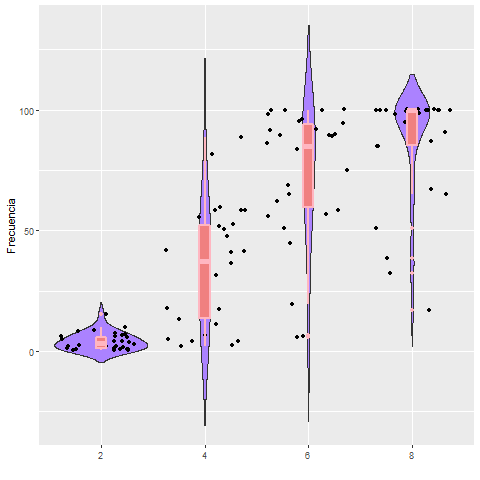
\includegraphics[width=0.5\textwidth]{t11_diagrama.png}
    \caption{Diagrama violín y caja-bigote de Pareto.}
    \label{fig1}
\end{figure}


\section{Conclusión}
A simple vista se puede deducir que se logra apreciar la tendencia al incremento conforme va aumentando el número de funciones objetivo, distribuyéndose así con la misma tendencia.

\bibliography{referencias}
\bibliographystyle{plainnat}


\end{document}